\section{Navigation Test}

The robot must enter the arena, visit each one from a set of waypoints, and leave the arena. The path from a waypoint to another is always blocked by an obstacle that requires the robot to take an action to solve the task.

Actions may include: avoid the obstacle, find a different path, or even interact with the obstacle (move it, open it, ask it to move, wait for it to move, etc.).

\subsection{Goal}
The robot must be able navigate through the apartment and avoid some difficult obstacles along the way.

\subsection{Focus}
The navigation test focuses on navigating in a changing environment, where doors can be closed and even paths to goal may get blocked by movable temporary objects. 

Perceiving the obstacles is also critical in safely navigating a home environment.

\subsection{Setup}

\begin{enumerate}
\item \textbf{Location:} One of the arenas (apartment). The apartment is in its normal state.
\item \textbf{Doors:} All doors in the apartment are open, except for the entry door. The arena/apartment must contain 2 doors within the apartment (thus excluding the entry/exit doors). Any destination in the room should be reachable via either door but not via any other way.
\end{enumerate}

\subsection{Task}
The robot must visit a set of waypoints and avoid the obstacles on its path. All waypoints are related to furniture in the arena, such as a table, a couch or a plant etc, and their order can be reversed.

\begin{enumerate}
\item \textbf{Entering the arena:} The robot starts outside the environment and must wait until the door opens.
\item \textbf{Waypoint A (door):} The robot must navigate to waypoint A. Waypoint A is reachable via several paths that include doors. One of the doors will be shut. The robot may:
\begin{enumerate}
\item To take a different path.
\item Open the closed door.
\end{enumerate}
The robot must report whether it reached the waypoint.

\item \textbf{Waypoint B (dynamic obstacles):} The robot must navigate to waypoint B which is also reachable via (the same) two doors, one of each may still be closed. On it's path the robot may find a dynamic obstacle (movable people, other robot, pets, etc.) which blocks it's path to waypoint B. The robot may:
\begin{enumerate}
\item To take a different path.
\item Ask the obstacle to move out.
\item Wait for the object to move away by itself.
\end{enumerate}
The robot must report whether it reached the waypoint.

\item \textbf{Waypoint 3 (following a human) [Optional]:} When requested by the team leader, there may be a \iterm{Professional Walker} waiting nearby Waypoint 2 (either A or B). Instead of just leaving the arena, the robot may follow the \iterm{Professional Walker} outside the arena to Waypoint 3 and then navigate back to the starting point.

\begin{enumerate}
\item \textbf{Memorizing the operator:} The robot has to memorize the operator. During this phase, the robot may instruct the operator to follow a certain setup procedure.
\item \textbf{Following the operator:} When the robot signals that it is ready to start, the operator is walking --in a natural way-- through a designated path outside the arena. The robot needs to follow the operator until the operator ask to the robot to stop doing so (Waypoint 3).
\item \textbf{Going back to the arena:} After following the operator, the robot must navigate back into the arena, though the same door for going out, till the point where it trained the operator.
\end{enumerate}

\item \textbf{Leave the arena:} Go outside the arena through the same the robot started.

\paragraph{Note} Objects will be placed during the test in the robot's path which it must avoid. The closing / opening doors give the Technical Committee the possibility to change the order in which the obstacles are encountered, so there is no predefined order of obstacles encountered. Again, waypoint A and B are interchangeable.
\end{enumerate}

\begin{figure}[tbp]
	\centering
	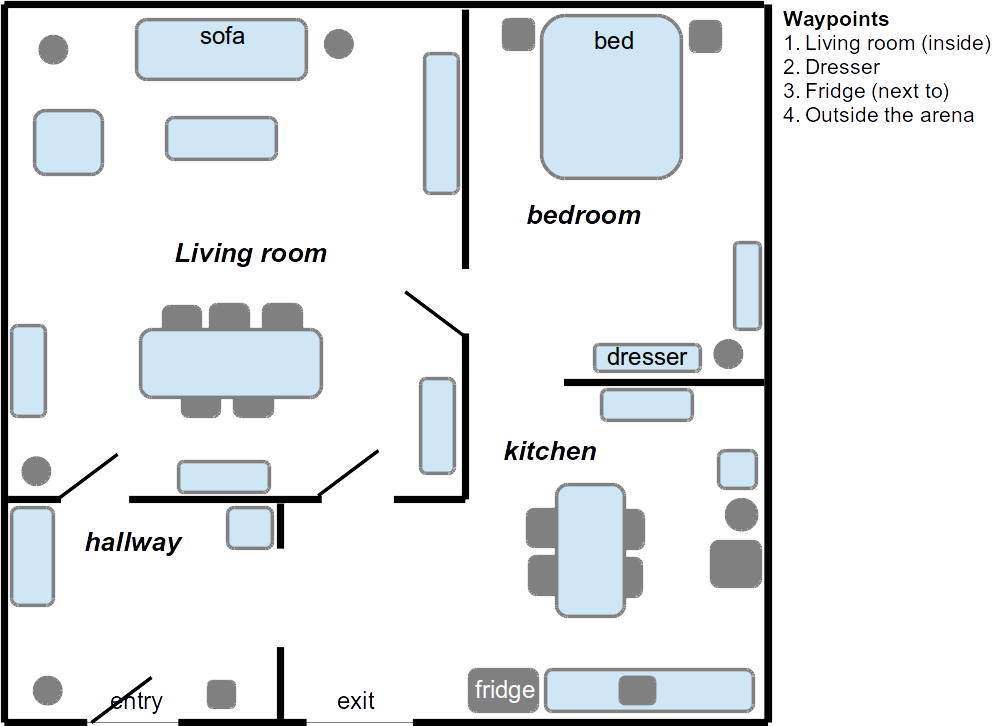
\includegraphics[width=0.75\columnwidth]{images/navigation.png}
	\caption{Navigation test waypoints.}
	\label{fig:navigation}
\end{figure}

\subsection{Additional rules and remarks}
\begin{enumerate}
	\item \textbf{Make it fast:} If a robot is absolutely unable to handle one or more obstacles, please inform the TC before the test so no time is wasted.
	\item \textbf{Closing doors:}  The door that will be shut will be the door on the route the robot has committed to. It will be shut right after the robot starts driving towards the door. The door will be closed well before the robot reaches it so the robot has enough time to notice that the door closed.
	\item \textbf{Obstacles:} obstacles may be:
	\begin{enumerate}
		\item [Obstacle 1:] Box sized item placed around a corner. 
		\item [Obstacle 2:] A static obstacle on or very near one of the waypoint. If the robot cannot reach the waypoint, it must report so by speech and continue the test. For example, a person may be standing in front of a couch and a chair may be placed at the table. 
		\item [Obstacle 3:] A bar table, normal table, rolling chair: some object that is wider at its top than on its bottom, thus requiring more than just a laser scanner mounted near the ground to avoid obstacles. This will be placed in the middle of some room, on or near the robots path.
	\end{enumerate}
	\item \textbf{Moving objects:} If the robot finds on it's way a \textit{static movable obstacle} (chair, cubes, toys, etc.) which is capable to move, it may move the object apart with it's manipulator.
	\item \textbf{When following people:} 
	\begin{enumerate}
		\item \textbf{Instruction:} The robot interacts with the operator, \emph{not} the team. That is, the team is not allowed to briefly instruct the operator.
		\item \textbf{Natural walking:} The operator has to walk \quotes{naturally}, i.e., move forward facing forward. The operator is not allowed to walk back, stand still, signal the robot or follow some re-calibration procedure.
		\item \textbf{Asking for passage:} The robot is allowed to (gently) ask people to step aside.
	\end{enumerate}
\end{enumerate}

%\subsubsection{Referee instructions}
%
%The referee needs to
%\begin{itemize}
%\item 
%\item 
%\end{itemize}

\subsection{Score sheet}

The maximum time for this test is 5 minutes.

\begin{scorelist}

	\scoreheading{Waypoints}
	\scoreitem{10}{Reaching waypoint A}
	\scoreitem{10}{Reaching waypoint B}

	\scoreheading{Obstacles}
	\scoreitem{20}{Avoiding obstacle 1}
	\scoreitem{30}{Avoiding obstacle 2}
	\scoreitem{40}{Avoiding obstacle 3}
	\scoreitem{10}{Reporting unreachable waypoint due to an obstacle (will end the test)}

	\scoreheading{Doors}
	\scoreitem[2]{20}{Starting a new path after reaching a closed door}
	\scoreitem[2]{45}{Opening the door and continue instead of plan a new trajectory}

	\scoreheading{Optional tasks (up to 50 points)}
	\scoreitem{10}{Reaching waypoint}
	\scoreitem{40}{Reentering the arena after reach Waypoint 3}

	\setTotalScore{200}
\end{scorelist}


% Local Variables:
% TeX-master: "Rulebook"
% End:


% Local Variables:
% TeX-master: "Rulebook"
% End:
